In \Cref{sec:reconstruction_overview} it was discussed that in about a half of all reconstructed events there exists more than one tag-side candidate.
That does not take into account the overlap between \feiBp and \feiBz mode -- which further enhances this effect.
Performing the best tag-side $B$ candidate selection is important, as multiple entries per event should not be included in the final sample.
However, the interest in this analysis lies in the signal side which decays as \BtoXsgamma, which means that a standard Belle II `truth-matching' procedure is too strict.
In principle, our requirement is to only reconstruct a sample of tag $B$ mesons that \textit{give provide good kinematic constraints to the signal side}.
In this section, these definition for best-candidate selection are discussed more broadly and
 a concrete definition for tag-$B$ mesons with correctly reconstructed kinematic properties is introduced.

\subsection{Selection within the same \texorpdfstring{\FEI}{FEI} mode}

The number of tag-side candidates for \feiBp and \feiBz modes, after the optimised selections in \Cref{tab:cutflow},
is shown in \Cref{fig:fei_tag_reco_candidates_post_optimisation}.
Overall, comparing to \Cref{fig:fei_tag_reco_candidates}, the candidate fractions are similar --
which attests to the fact that background (and particularly continuum) suppression was done without introducing a bias in preferentially selecting events with large \feiProb in \Cref{sec:continuum_suppression,sec:photon_selection}.

\begin{figure}[htbp!]
    \centering
    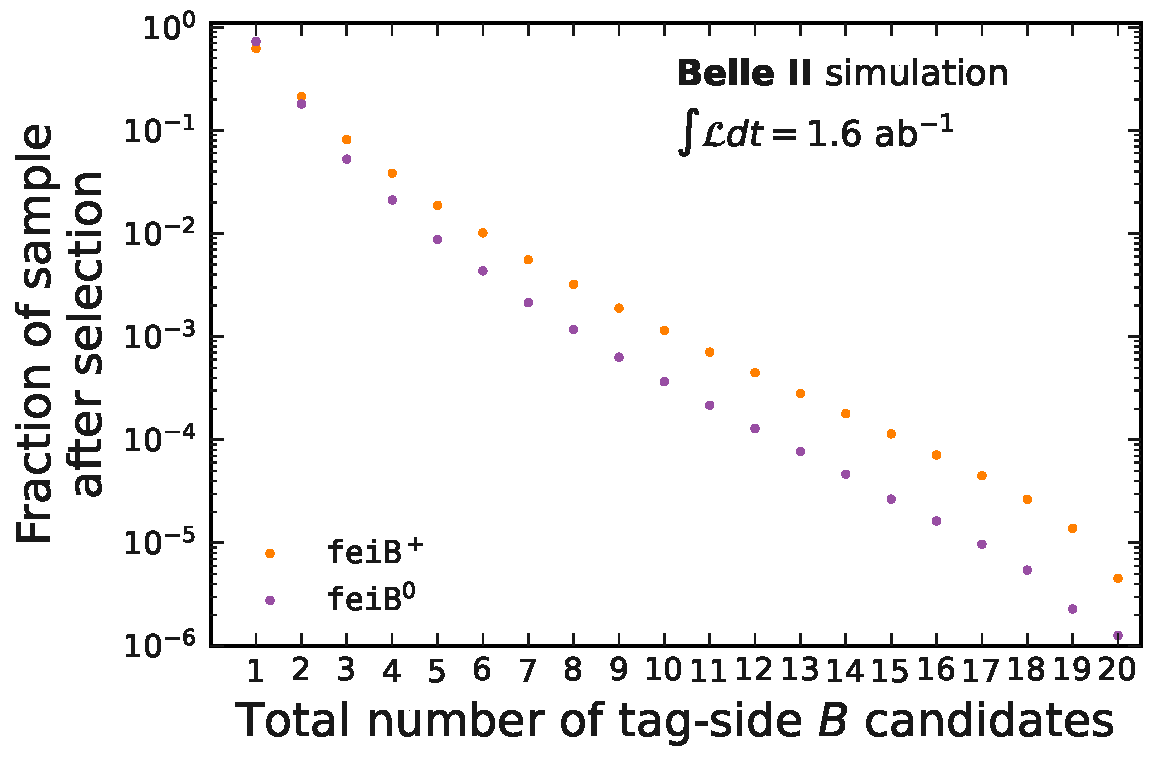
\includegraphics[width=0.45\textwidth]{figures/event_reconstruction/Bboth_total_tag_candidates.pdf}

    \caption{\label{fig:fei_tag_reco_candidates_post_optimisation} 
    Relative fractions of events for the number of \B meson candidates in the generic \MC dataset after the background suppression selections in \Cref{tab:cutflow}.
    This figure can be directly compared with \Cref{fig:fei_tag_reco_candidates}.
    The overall fractions are similar.
    About 67\%(74\%) of events for \Bp and \Bz \FEI modes have only 1 tag-side candidate.
    About 19\%(17\%) of events for \Bp and \Bz \FEI modes have two tag-side candidates and 7\%(5\%) has 3.
    The number of candidates per event reduces quickly, but faster for \Bz modes, with roughly 2\%(1\%) of events having more than 5 candidates for \Bp and \Bz.
    Note that the same event can have a \Bp and \Bz event reconstructed.
    }
\end{figure}

It is clear, however, that even after all selections there may still exist more than one \B meson + photon combination.
The first step in this is a selection of best-tag-candidate per \FEI mode, i.e. the best candidate between \feiBp and \feiBz modes.
While a general approach could be developed, it was observed that at this stage a particular choice of the tag does not influence the resolution or the average value of the spectrum strongly.
This is visualised in \Cref{fig:same_mode_best_tag_selection}.
For both neutral and charged \BtoXsgamma modes the distributions look similar whether the highest-\feiProb candidate is selected in each event, or a random tag-$B$ meson is chosen as the main candidate.
On the other hand, the \Mbc distribution, as expected, has a higher peak for the case when the highest \feiProb candidate is picked in each event.
The latter result for \BtoXsgamma is shown in \Cref{fig:same_mbc_best_tag_selection}.
The figure also includes a similar \Mbc test for the continuum events.

\begin{figure}[htbp!]
    \subcaptionbox{\label{fig:bp_same_mode_best_tag_selection}}{
        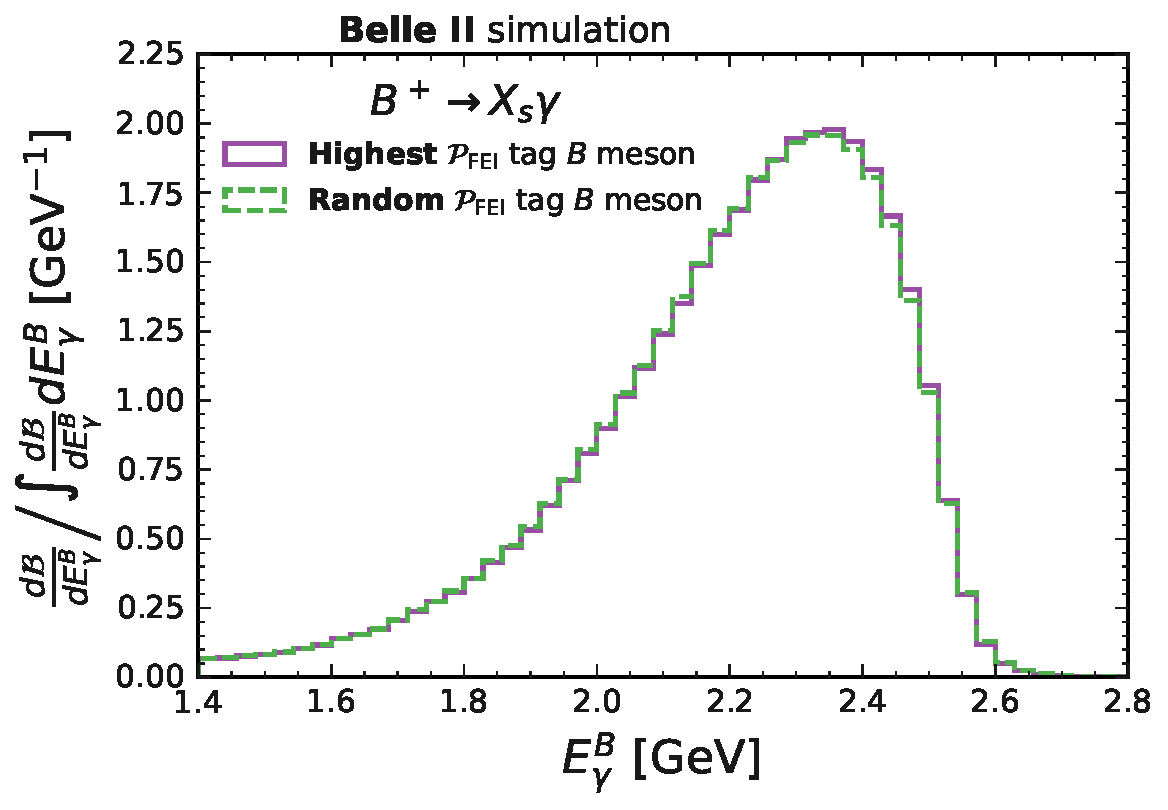
\includegraphics[width=0.4\textwidth]{figures/best_tag_selection/bp_spectrum_with_random_best_tag_selection.pdf}
    }
    \subcaptionbox{\label{fig:bz_same_mode_best_tag_selection}}{
        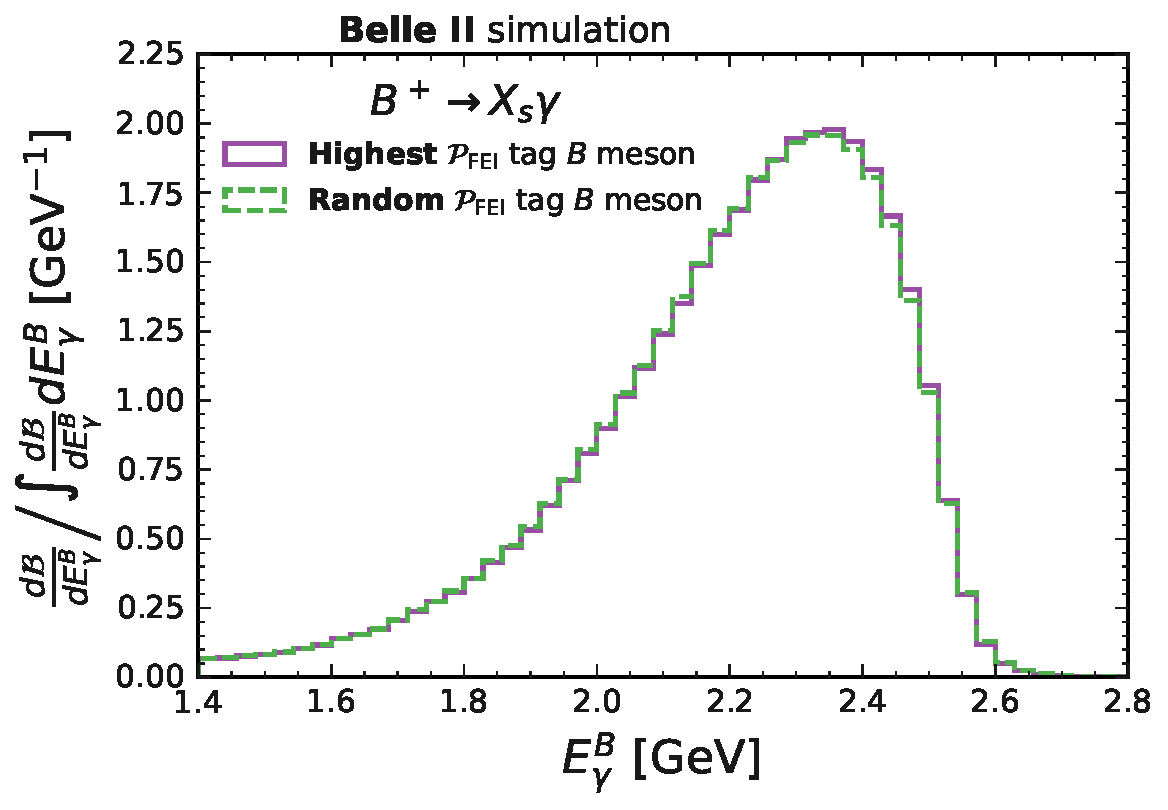
\includegraphics[width=0.4\textwidth]{figures/best_tag_selection/bp_spectrum_with_random_best_tag_selection.pdf}
    }
    \caption{\label{fig:same_mode_best_tag_selection}Photon energy spectrum (\Cref{fig:bp_same_mode_best_tag_selection}) after selecting a single tag $B$ meson candidate per event either randomly or by requiring the largest \feiProb.
    This is shown for \BptoXsgamma events in \Cref{fig:bp_same_mode_best_tag_selection} 
    and \BztoXsgamma in \Cref{fig:bz_same_mode_best_tag_selection}.
    The figures are normalised to their total integral value such that a shape comparison can be performed.
    Overall, the difference in resolution is small and evaluated at about \order(0.1\%), which is at least an order of magnitude smaller than expected statistical precision of the analysis.
    \todo[inline]{ref resolution chapter}.
    }
\end{figure}

\begin{figure}[htbp!]
    \centering
    \subcaptionbox{\label{fig:bp_mbc_mode_best_tag_selection}}{
        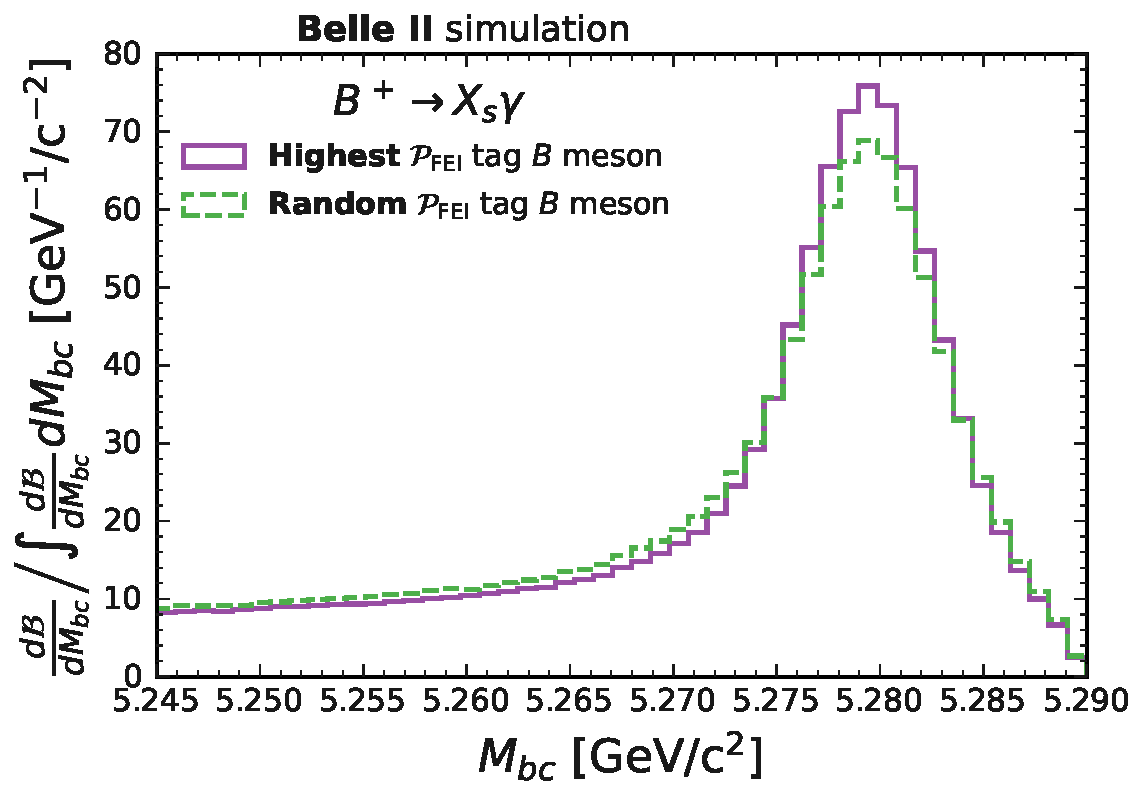
\includegraphics[width=0.4\textwidth]{figures/best_tag_selection/bp_Mbc_with_random_best_tag_selection.pdf}
    }
    \subcaptionbox{\label{fig:bz_mbc_mode_best_tag_selection}}{
        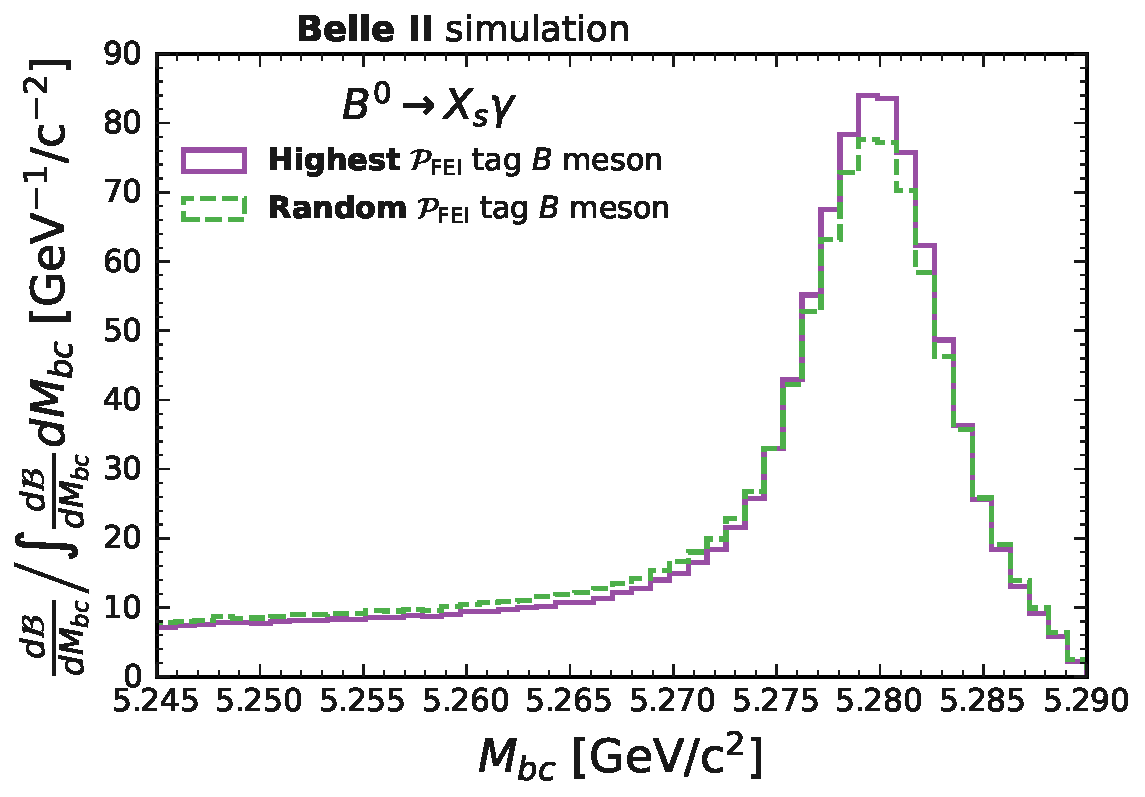
\includegraphics[width=0.4\textwidth]{figures/best_tag_selection/bz_Mbc_with_random_best_tag_selection.pdf}
    }
    \subcaptionbox{\label{fig:bp_continuum_mode_best_tag_selection}}{
        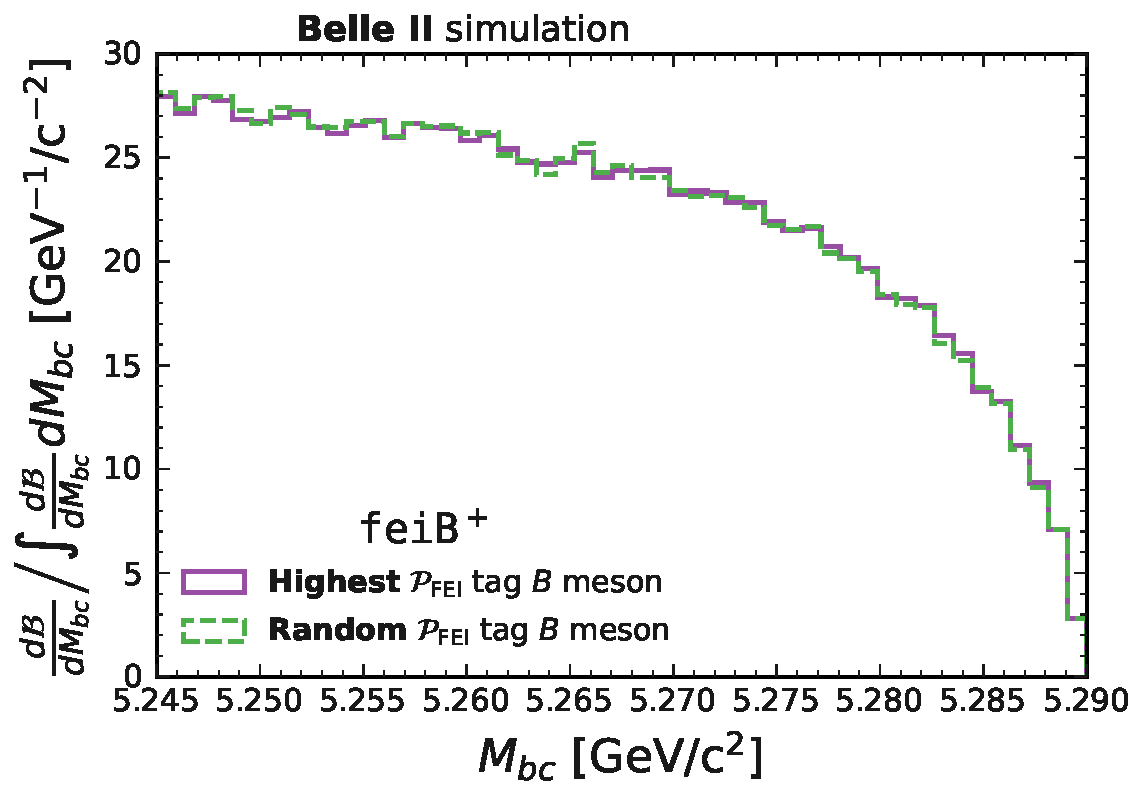
\includegraphics[width=0.4\textwidth]{figures/best_tag_selection/bp_continuum_Mbc_with_random_best_tag_selection.pdf}
    }
    \subcaptionbox{\label{fig:bz_continuum_mode_best_tag_selection}}{
        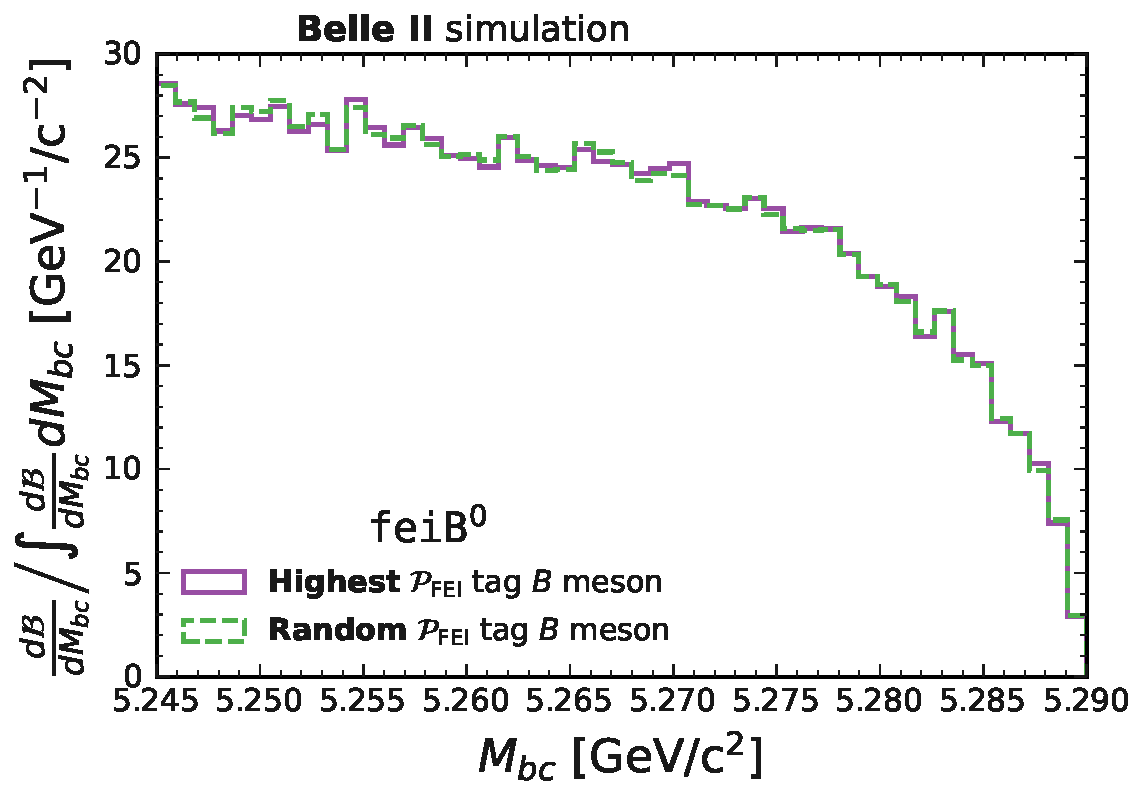
\includegraphics[width=0.4\textwidth]{figures/best_tag_selection/bz_continuum_Mbc_with_random_best_tag_selection.pdf}
    }
    \caption{\label{fig:same_mbc_best_tag_selection}\Mbc shapes for \BtoXsgamma signal \MC (\Cref{fig:bp_mbc_mode_best_tag_selection,fig:bz_mbc_mode_best_tag_selection}) 
    and \mbox{\epem\ra\qqbar} events from generic-\MC (\Cref{fig:bp_continuum_mode_best_tag_selection,fig:bz_continuum_mode_best_tag_selection}) after selecting a single tag $B$ meson candidate per event either randomly or by requiring the large \feiProb.
    \Cref{fig:bp_mbc_mode_best_tag_selection,fig:bp_continuum_mode_best_tag_selection} show that the difference in the \Mbc distribution for \BptoXsgamma and \BztoXsgamma mostly pronounced in the peak region.
    On the other hand, \Cref{fig:bp_continuum_mode_best_tag_selection,fig:bz_continuum_mode_best_tag_selection} shows not strong dependance in shape irrespective of the way the tag-side candidate is chosen.
    The figures are normalised to their total integral value such that a shape comparison can be performed.
    This observation motivates to selected the highest-\feiProb candidate.
    }    
\end{figure}

As it is desirable to emphasise the contrast between continuum and $B$ events for the fitting step that will follow (see XXX)
\todo[inline]{XXX}
the highest \feiProb candidate in each event is chosen as the $B$ candidate with virtually no bias to the resolution.
However, the study here, as of yet, does not address the cases when there is a candiate in the same event reconstructed in \feiBp and \feiBz.
Therefore, for now, both candidates are kept in such events and the study is continued in \Cref{sec:select_best_candidate}.

\subsection{Selection between \texorpdfstring{\feiBp}{feiB+} and \texorpdfstring{\feiBz}{feiB0} mode}\label{sec:select_best_candidate}

The last section showed that one can select the highest \feiProb candidate from \feiBp and \feiBz without a significant effect on the \EB resolution, and with an enhancement of the \Mbc distribution peak.
As such it reduced each event to a signle tag-$B$ and photon combination in most events.
However, it did not address the case when there is a candidate reconstructed in both \feiBp and \feiBz modes: implying that events may still have up to two combinations.
Such cases are evaluated to happen roughly 10.5\% of time. 
For the sample where two $B$ candidates exist, two quantities are calculated
\begin{equation}\label{eq:asymmetry_tag}
    \mathcal{A}_{\mathrm{tag}} = \frac{\mathcal{P}_{\mathrm{tag}}(\feiBp) - \mathcal{P}_{\mathrm{tag}}(\feiBz)}{\mathcal{P}_{\mathrm{tag}}(\feiBp) + \mathcal{P}_{\mathrm{tag}}(\feiBz)},
\end{equation}
which is called the asymmetry of \feiProb between a \feiBp and \feiBz candidate in the same event, and
\begin{equation}\label{eq:delta_mbc}
    \Delta(\Mbc) = \Mbc(\Bp) - \Mbc(\Bz),
\end{equation}
which is the difference in \Mbc value of the two candidates.
The $\mathcal{A}_{\mathrm{tag}}$ tends to zero if they both have a similar \feiProb and to $\pm$ unity if one of the candidates has a much larger \feiProb.
The second $\Delta(\Mbc)$ is a difference in \Mbc between both of the candidates.
These quantities are visualised in a two-dimensional grid in \Cref{fig:selecting_tag_mode}.
In the figure, the sample is split into two samples, where a real \Bp or \Bz hadronic decay is present on the tag-side, in \Cref{fig:bp_selecting_tag_mode} and \Cref{fig:bz_selecting_tag_mode}, respectively.
If a $\Bp$ candidate is present $\mathcal{A}_{\mathrm{tag}}\approx1$ and $\Delta(\Mbc)\gtrsim 0$ for majority of the candidates.
For $\Bz$ candidates the opposite is true: $\mathcal{A}_{\mathrm{tag}}\approx-1$ and $\Delta(\Mbc)\lesssim 0$ for majority of the candidates.
This result implies that if the true candidate is a \Bp(\Bz), then the value of \feiProb will be higher from \feiBp (\feiBz) candidates the opposite \FEI mode.
Furthermore, the fact that $\Delta(\Mbc)$ tends to be higher can simply be understood that the incorrect candidate is more likely to be present in the tail, rather than peak region of \Mbc.

\begin{figure}[htbp!]
    \centering
    \subcaptionbox{\label{fig:bp_selecting_tag_mode}}{
        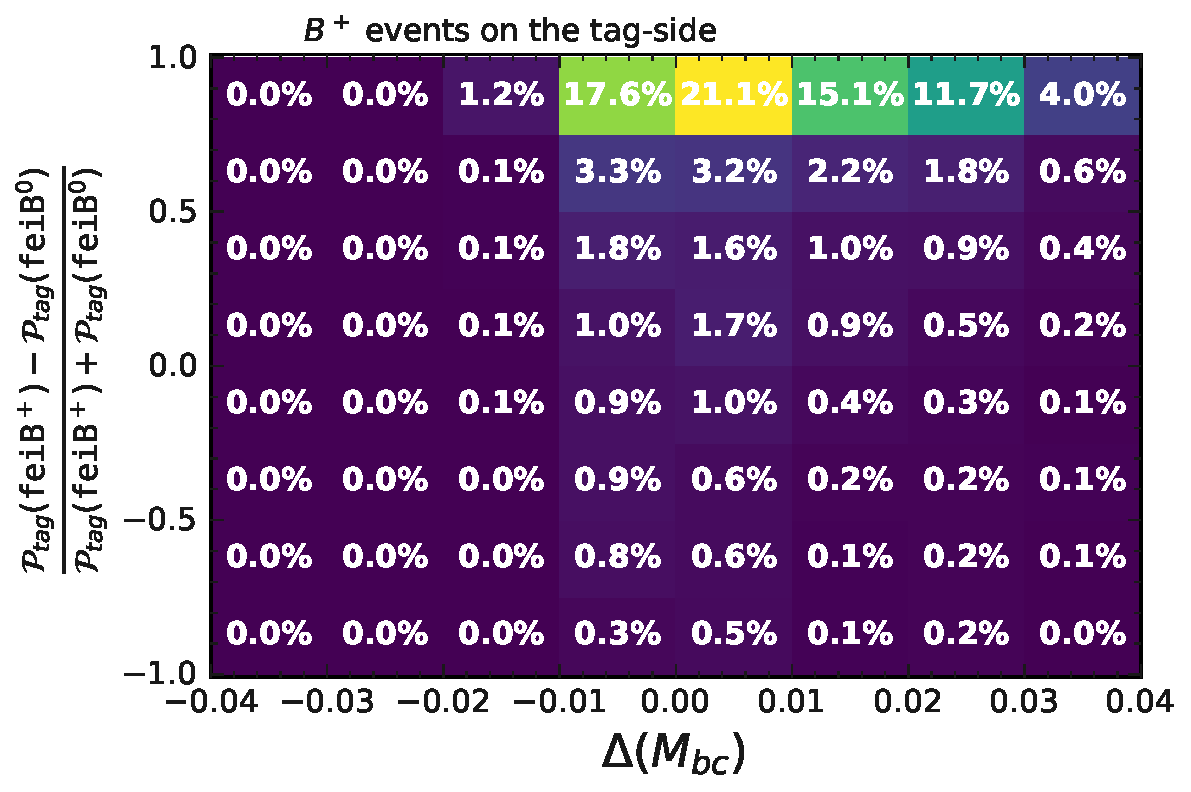
\includegraphics[width=0.4\textwidth]{figures/best_tag_selection/Bp_selecting_between_bp_bz.pdf}
    }
    \subcaptionbox{\label{fig:bz_selecting_tag_mode}}{
        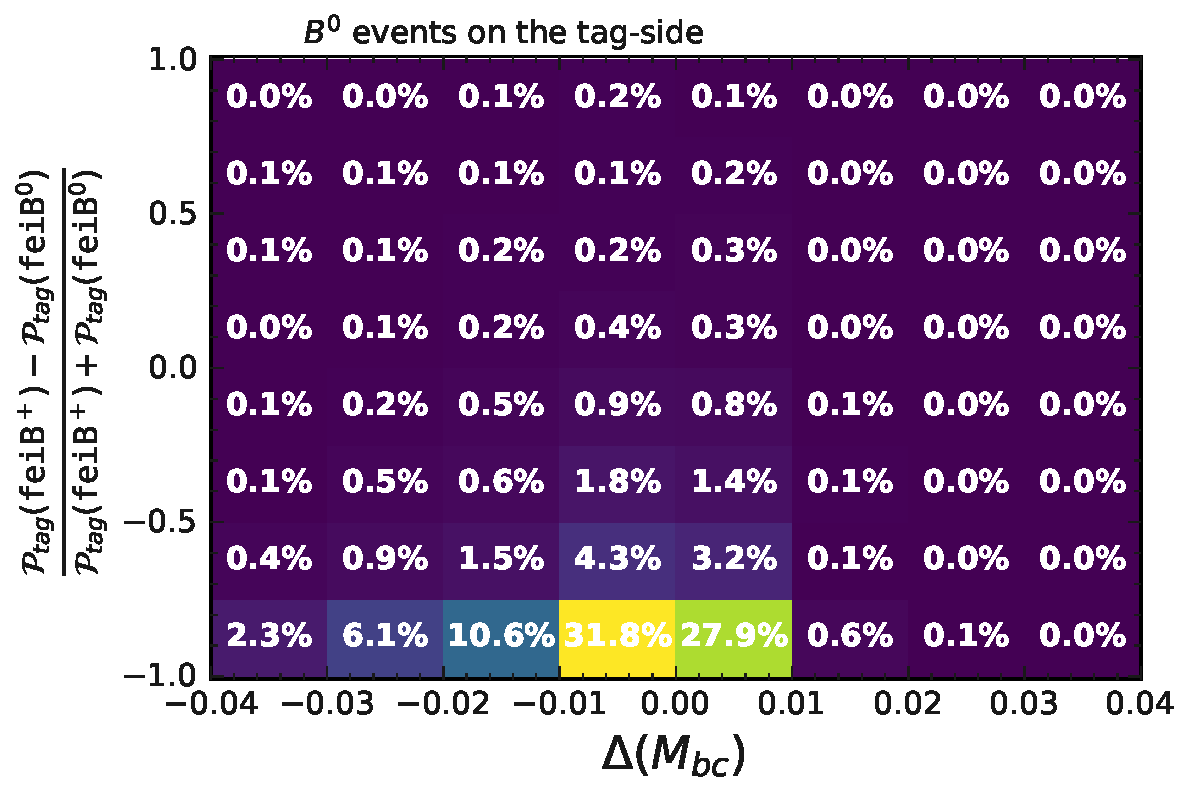
\includegraphics[width=0.4\textwidth]{figures/best_tag_selection/Bz_selecting_between_bp_bz.pdf}
    }
    \caption{\label{fig:selecting_tag_mode} A two-dimensional grid of $\mathcal{A}_{\mathrm{tag}}$ (\Cref{eq:asymmetry_tag})
    and $\Delta(\Mbc)$ (\Cref{eq:delta_mbc}) for events that have 2 $B$ candidates from \feiBp and \feiBz modes.
    Candidates with a real tag-side $B^+$ decay (\Cref{fig:bp_selecting_tag_mode})
    and a real tag-side $B^0$ decay (\Cref{fig:bz_selecting_tag_mode}) are shown.
    Most candidates lie near $\mathcal{A}_{\mathrm{tag}}\approx +1 (-1)$ and.
    $\Delta(\Mbc)$ value tends to be positive (negative) for $\Bp(\Bz)$ candidates.
    }
\end{figure}

Based on the observations discussed in this sections, it can be concluded that it is appropriate to select the \FEI candidate with the highest signal probability even when selecting between different \feiBp and \feiBz modes.
This selections finalises the best-candidate selection in this analysis as now it is ensured that every photon candidate corresponds to a single, unique tag-side $B$ meson candidate.

\subsection{Estimation of kinematically-consistent \texorpdfstring{$B$}{B}-meson}\label{sec:good_tag_definition}
